\documentclass[12pt]{article}

\include{../style}

\begin{document}

\title{Cosc 30: Discrete Mathematics}

\author{Prishita Dharampal}
\date{}
\maketitle
\vspace{-0.3in}


\begin{problem}{1}
    \textbf{Vector Racer. [Erickson Chap. 5, Ex. 25]} 
    
    Vector Racer is a two-player paper-and-pencil racing game.1 The game is played with a track drawn on a sheet of graph paper. The players alternately choose a sequence of grid points that represent the motion of a car around the track, subject to certain constraints explained below: 
    
    \begin{center}
            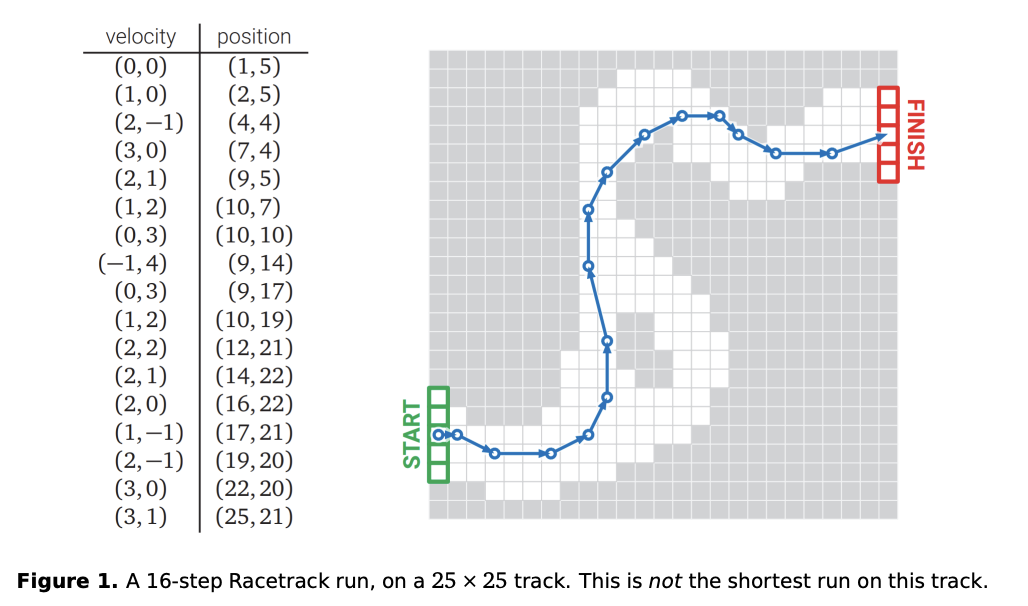
\includegraphics[width=0.5\linewidth]{assests/S1.png}
    \end{center}
    
    Each car has a position and a velocity, both with integer x- and y-coordinates. A subset of grid squares is marked as the starting area, and another subset is marked as the finishing area. The initial position of each car is chosen by the player somewhere in the starting area; the initial velocity of each car is always (0,0). At each step, the player optionally increments or decrements either or both coordinates of the car’s velocity; in other words, each component of the velocity can change by at most 1 in a single step. The car’s new position is then determined by adding the new velocity to the car’s previous position. The new position must be inside the track; otherwise, the car crashes and that player loses the race. (For sake of simplicity, we allow the “glitch” that the car can pass through obstacles that are not on tracks when there is enough velocity.) The race ends when the first car reaches a position inside the finishing area.
    
    Suppose the racetrack is represented by an $n \times n$ array of bits, where each $0$ bit represents a grid point inside the track, each $1$ bit represents a grid point outside the track, the “starting area” is the first column, and the “finishing area” is the last column.
    
    \begin{enumerate}
    \item[(a)] Construct a graph $G$ and describe an equivalent problem on $G$, including the input and output, for the following problem: Find the minimum number of steps required to move a car from the starting line to the finish line of a given racetrack.
    
    \item[(b)] Prove that in a run with minimum number of steps from start to finish, the car will never be at the exactly same position and have the same velocity twice. (To think about later: Oh a shortest route, can the car be at the exactly same position twice where the velocity could be different?)
    \end{enumerate}
\end{problem}

\begin{problem}{2}
    \textbf{Needles on the ground.} 
    
    Fix a collection of line segments in the plane. Without loss of generality we assume no two line segments are parallel. This implies that given any two line segments, either they are disjoint, or they have a unique crossing. We also assume no three or more segments intersect at a common point; this can be achieved by slightly perturbing the segments.
    
    A collection of line segments partitions the plane into connected regions, each of which is a maximally connected component in the plane subtracting the line segments. The size of a region is the number of crossings on the boundary of the region. Notice that the same crossing may show up multiple times on the boundary; in this case we count its multiplicity.

     \begin{center}
            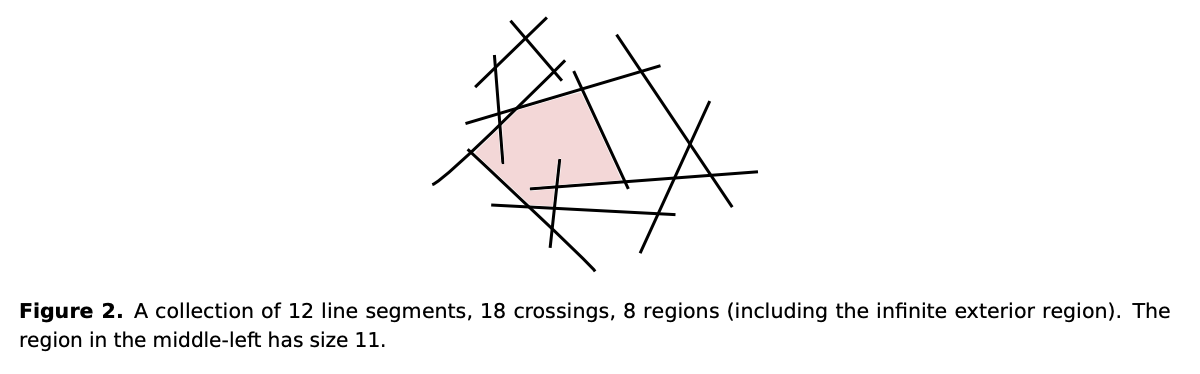
\includegraphics[width=0.5\linewidth]{assests/S2.png}
    \end{center}
    Prove that given an arbitrary collection of $n$ line segments, some segment has few crossings. Specifically, there is a segment that intersects at most
    \[
    \frac{\sum_{\text{region } R} |R|}{2n}
    \]
    other line segments, where $|R|$ is the size of the region $R$.
\end{problem}

\begin{problem}{3}
    A graph is regular if all its vertices have the same degree. Prove that every $n$-node simple regular graph $G$ with at least $n^2/4$ edges must be connected.
    
    [You really need the simpleness. Can you come up with a counter-example if the graph is not simple?]
\end{problem}
\end{document}